\documentclass{beamer}	
\mode<presentation>
 
\usepackage{pdfpages}
\usepackage{fancyvrb}
\usepackage{chemarr}

\usepackage{amsmath}		%% mathematics typesetting
\usepackage{amssymb}
 
\usepackage{epigraph}   %% nice setting of quotations

\usepackage{tabularx} %% allows to use row colours in tables

\usepackage{ulem}

\usepackage{booktabs}

\usepackage{siunitx} %% tpyeset SI units

\usepackage{CJKutf8} %% typeset Chinese characters

\usepackage{pdfpages}%% include pdfs


\usepackage{animate} %% show animated gifs

\DeclareMathAlphabet{\mathcalligra}{T1}{calligra}{m}{n}


% Color and Theme. Can be changed. However, this one's quite nice.
\usetheme{Madrid}
\definecolor{theme}{rgb}{0.84,0,0.21}
\usecolortheme[named=theme]{structure}


%%  Title information
\title[M11.10.3 Schwangerschaft]{M11.10.3 Sexualentwicklung und Reproduktionsphysiologie II: Schwangerschaft}
\author[melanie.stefan@medicalschool-berlin.de]{}
\institute[]{Prof. Melanie Stefan - melanie.stefan@medcialschool-berlin.de}
\date{SoSe 2022}
 

% Table of contents to pop up at the beginning of each section
\AtBeginSection[]
{
  \begin{frame}<beamer>
    \frametitle{Outline}
    \tableofcontents[currentsection,currentsubsection]
  \end{frame}
}
 
\beamertemplatenavigationsymbolsempty

\begin{document}


{
  \usebackgroundtemplate{
\includegraphics[width=1.2\paperwidth]{MSB_Titelseite.pdf}} 
\begin{frame}

 \maketitle 

$\,$\\[6cm]


\end{frame} 
}



%% Hook: 

\begin{frame}

\begin{center}

\includegraphics[width=\textwidth]{supreme_court_abtreibung.png}
\end{center}

\end{frame} 



%% %% TLIA

 
\begin{frame}
\frametitle{In dieser Vorlesung geht es um\dots}


\begin{columns}[c]
\begin{column}{5cm}
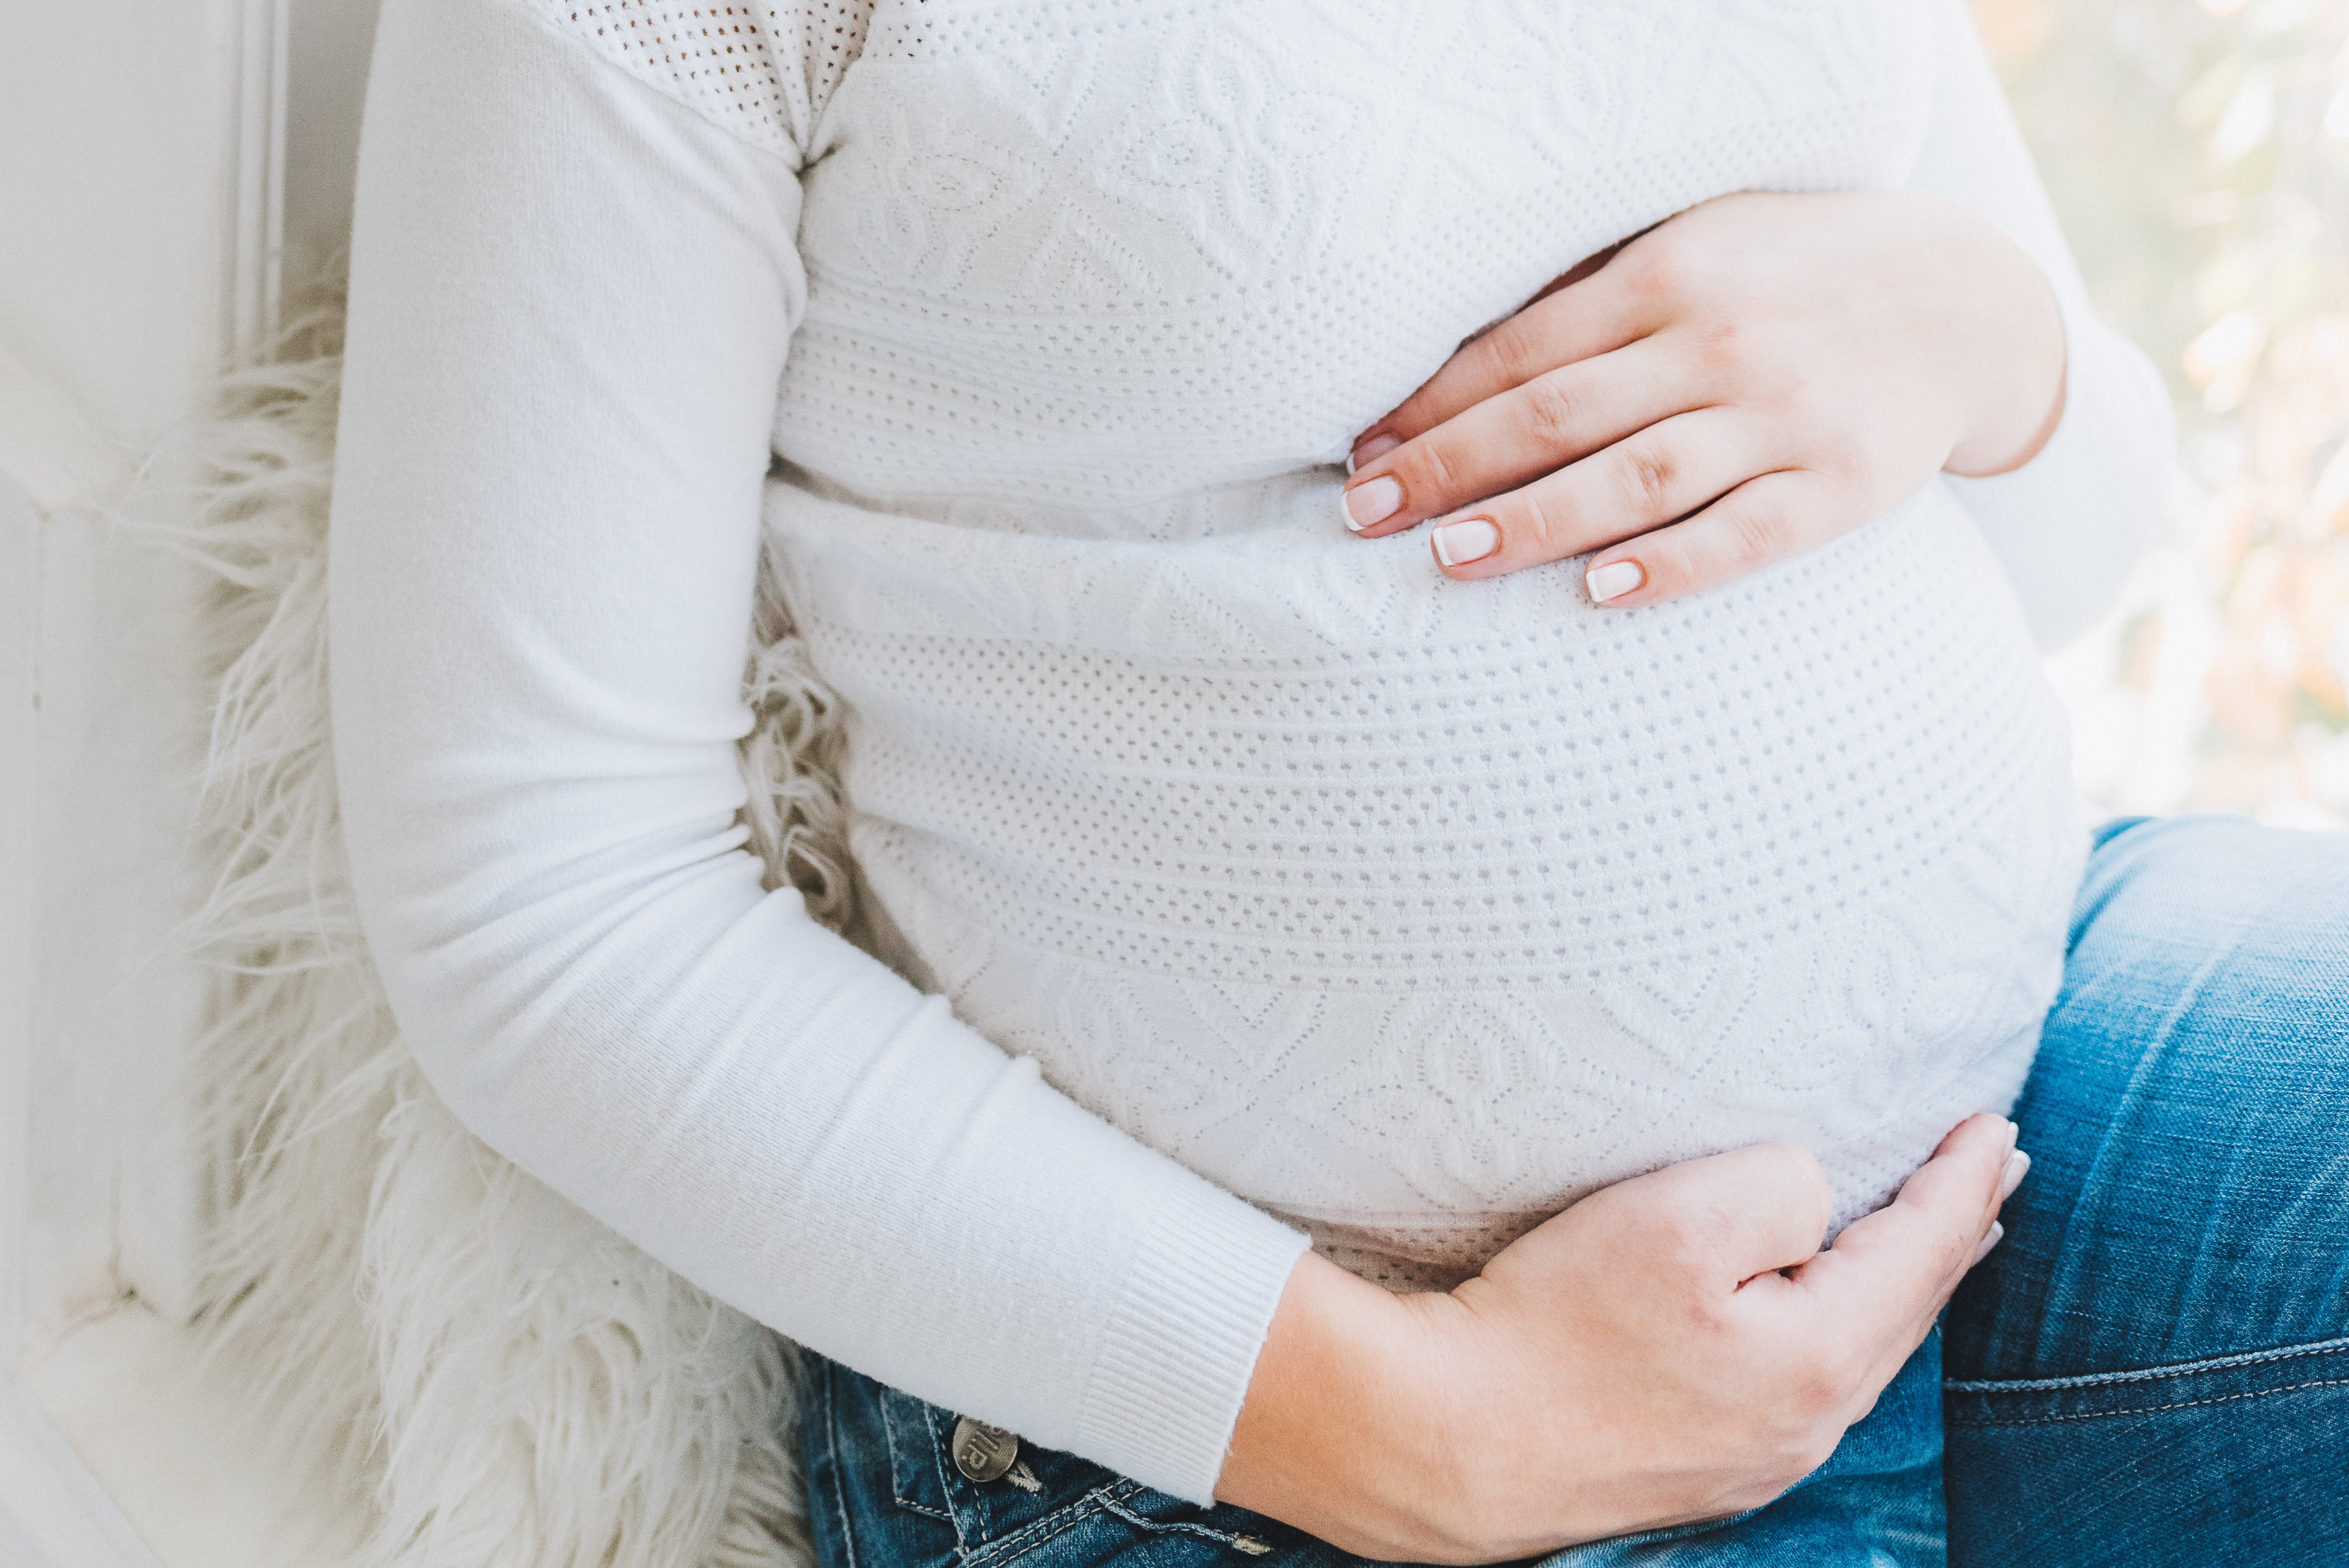
\includegraphics[width=\textwidth]{schwangerer_bauch.jpg}

\end{column}

\begin{column}{6cm}

\dots Schwangerschaft, \\ 
Entwicklung von Embryo und Fötus, \\
Geburt und Stillen

\end{column}
\end{columns}






\end{frame} 


%% %% Learning Objectives
 
\begin{frame}

 \frametitle{Nach dieser Vorlesung sollten Sie folgendes können}



\begin{block}{Grundlagen:}
\begin{itemize}
\item
Hormonelle Veränderungen im Verlauf der Schwangerschaft beschreiben und erklären
\item
die Entwicklung des Embryos und Fötus erklären 
\item
Körperfunktionen und Stoffaustausch des Fötus beschreiben
\item
die "Fetoplazentare Einheit" und Funktion der Plazenta erläutern
\item
den Geburtsvorgang beschreiben und erklären
\item
die hormonelle Steuerung der Laktation erklären

\end{itemize}

\end{block}



\begin{block}{Klinik:}
\begin{itemize}
\item
Erklären, wie ein Schwangerschaftstest funktioniert
\item
häufige Beschwerden und Komplikationen in der Schwangerschaft erklären

\end{itemize}

\end{block}

\end{frame}


%% %% %% Main Body




 

\section{Keimstadium, Nidation}


%% Keimstadium bis zur Einnistung
\begin{frame}
\frametitle{Während der ersten Zellteilungen wandert der Embryo in den Uterus}

\begin{center}
\includegraphics<1>[width=0.8\textwidth]{Human_Fertilization_Day0A.png}

\includegraphics<2>[width=0.8\textwidth]{Human_Fertilization_Day0B.png}

\includegraphics<3>[width=0.8\textwidth]{Human_Fertilization_Day0C.png}

\includegraphics<4>[width=0.8\textwidth]{Human_Fertilization_Day1.png}

\includegraphics<5>[width=0.8\textwidth]{Human_Fertilization_Day2.png}

\includegraphics<6>[width=0.8\textwidth]{Human_Fertilization_Day3A.png}

\includegraphics<7>[width=0.8\textwidth]{Human_Fertilization_Day3B.png}

\includegraphics<8>[width=0.8\textwidth]{Human_Fertilization_Day4.png}

\includegraphics<9>[width=0.8\textwidth]{Human_Fertilization_Day5.png}

\includegraphics<10>[width=0.8\textwidth]{Human_Fertilization_Day6.png}

\includegraphics<11>[width=0.8\textwidth]{Human_Fertilization.png}

\end{center}


\end{frame}


\begin{frame}
\frametitle{Komplikation: Ektopische Schwangerschaft im Eileiter}


\begin{columns}[c]
\begin{column}{5cm}

\begin{itemize}

\item
Embryo gelangt nicht in den Uterus, sondern nistet sich im Eileiter ein
\item
Wenn nicht erkannt,  kommt es  einem spontanen Abbruch oder einer (gefährlichen) Eileiter-Ruptur
\item
Wenn erkannt, muss die Schwangerschaft beendet werden
\end{itemize}

\end{column}

\begin{column}{5cm}

\begin{center}
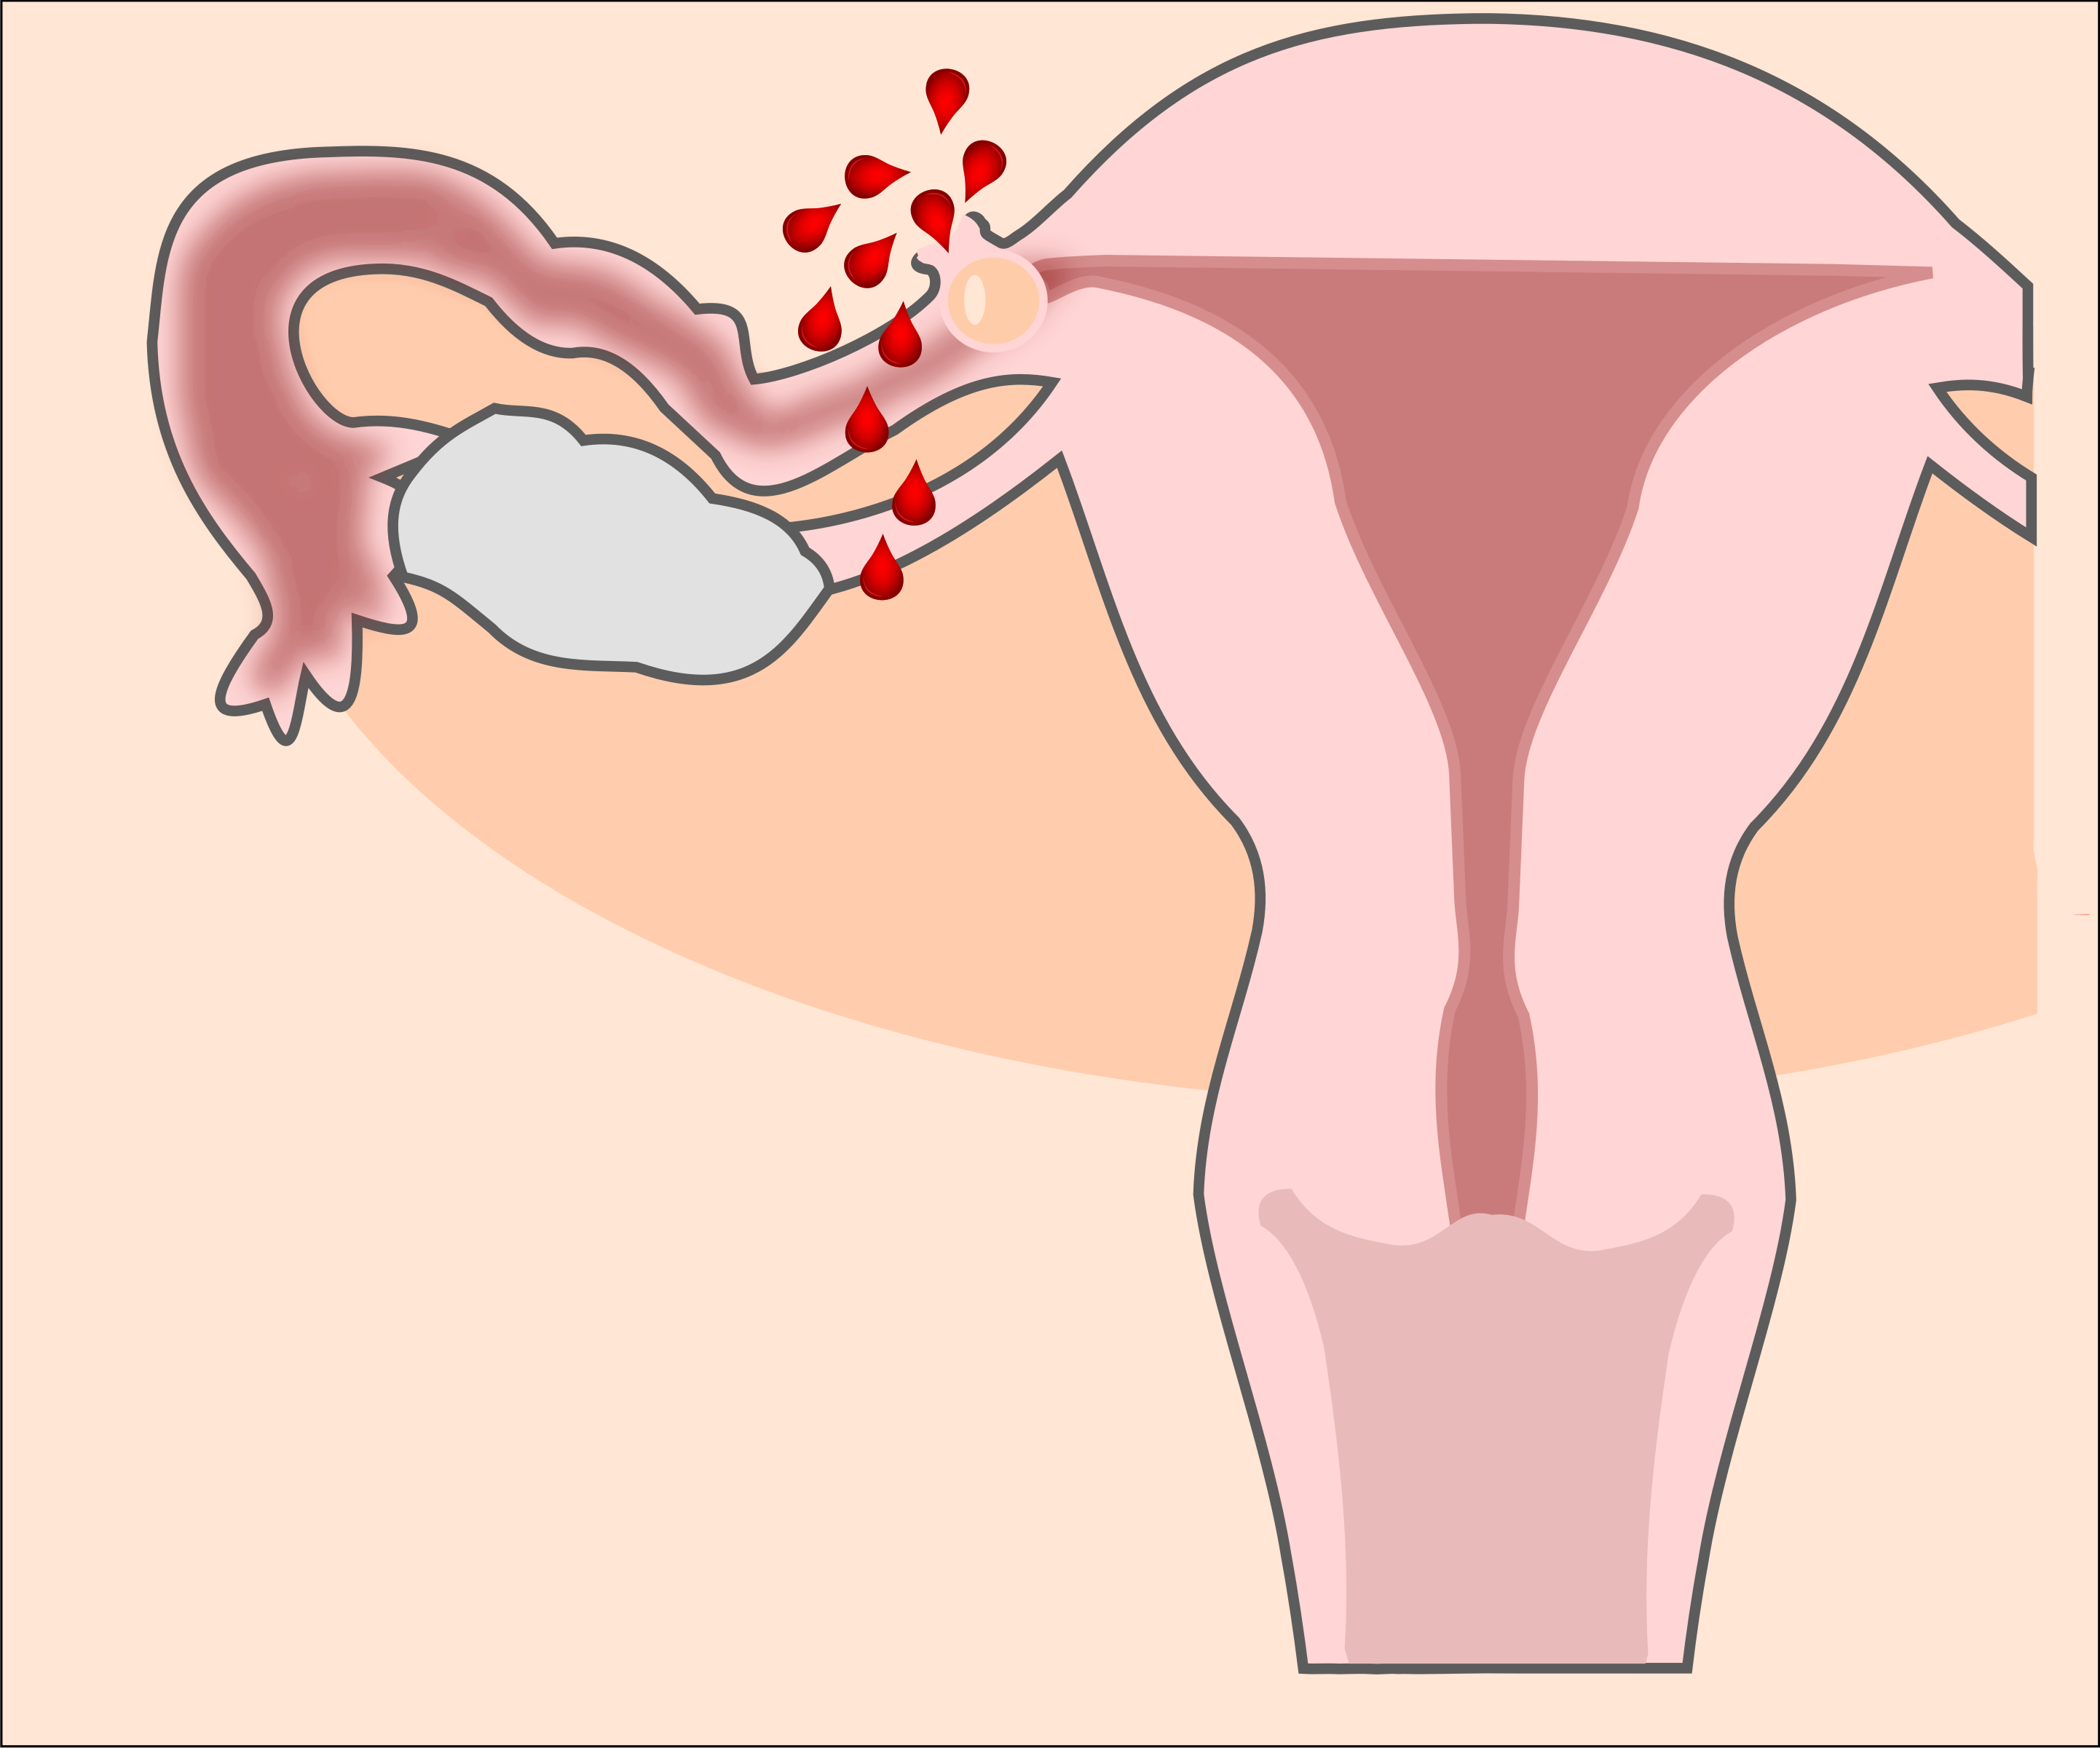
\includegraphics[width=\textwidth]{Eileiterruptur.png}
\end{center}


\end{column}
\end{columns}


\end{frame}

\section{Embryonalstadium}

\begin{frame}
\frametitle{Der  eingenistete Embryo produziert hCG}

\begin{itemize}
    \item 
    humanes Choriongonadotropin (hCG)
    \item 
    sehr ähnlich wie LH
    \item
    Stimuliert die Progesteronbildung im Corpus luteum gravitas
    \item
    Aufrechterhaltung der Schwangerschaft
    
\end{itemize}


\end{frame}


\begin{frame}
\frametitle{Bei Schwangerschaftstests wird auf hCG getestet}

\begin{columns}[c]



\begin{column}{5cm}
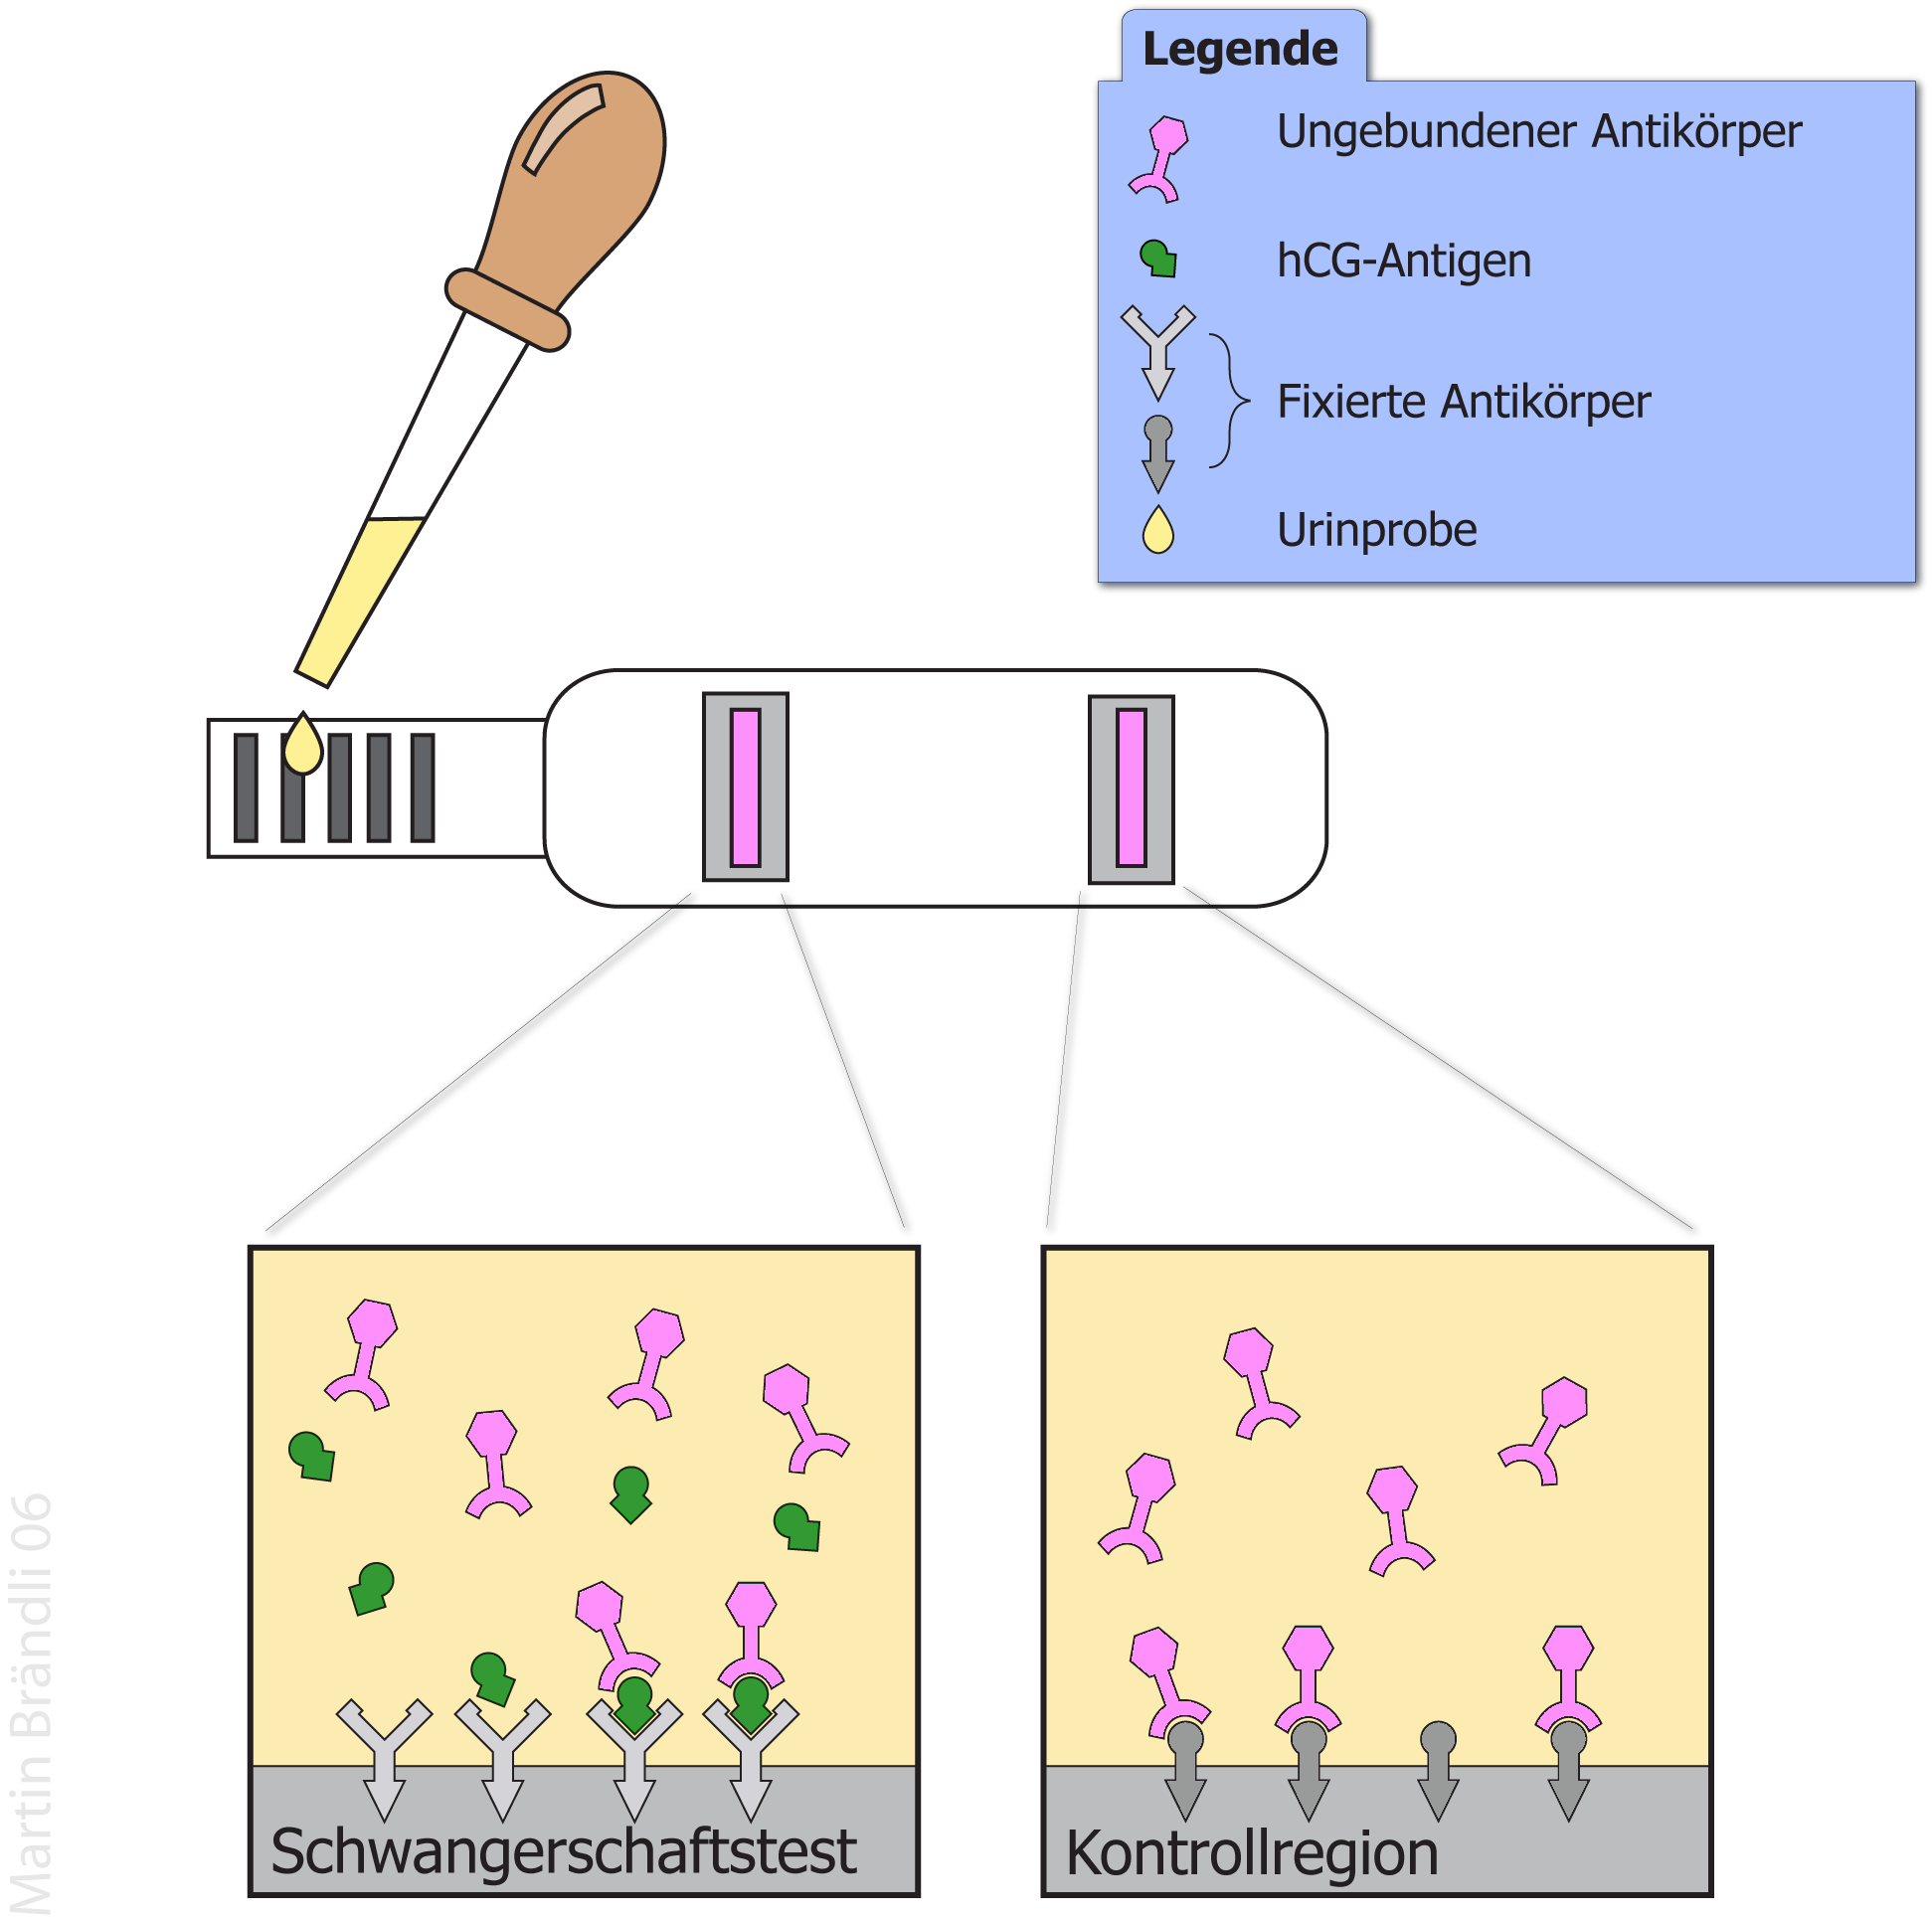
\includegraphics[width=\textwidth]{Schwangerschaftstest_Schema.png}
\end{column}


\begin{column}{5cm}

Nachweisbar im Urin: Ab 12-14 Tage nach Befruchtung

\pause



\end{column}

\end{columns}

\end{frame}



%% Blastozyste Embryoblast Trophoblast

\begin{frame}
\frametitle{Teile der Blastozyste haben unterschiedliche Funktionen}

\begin{columns}[c]

\begin{column}{5cm}
\begin{center}
    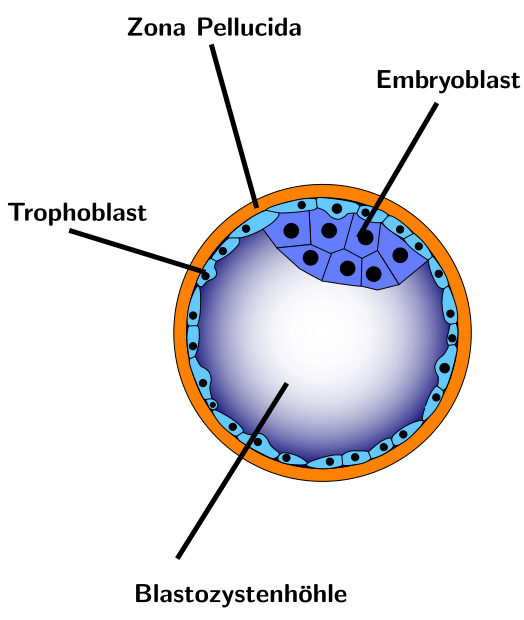
\includegraphics[width=\textwidth]{Blastozyste.png}
\end{center}
\end{column}

\begin{column}{5cm}

Aus dem Embryoblast entwickelt sich der Embryo. \\[0.2 cm]

Aus dem Trophoblast entwickelt sich Syncytiotrophoblast und Zytotrophoblast (später: Plazenta)

\end{column}

\end{columns}

\end{frame}


%% Gastrulation
%% Keimblaetter
%%\begin{frame}{Durch die Gastrulation bilden sich die Keimblätter }
    
%% \end{frame}


%% Primitivstreifen

%% Veraenderungen in der Schwangeren


%% Ende der Embryonalphase

\section{Fetalstadium}

\section{Geburt}

\begin{frame}
\frametitle{Geburtsphasen }

\begin{block}{Einleitung}
\begin{itemize}
\item
nach ca.  40 Schwangerschaftswochen
\item
Oxytozin und Prostaglandine bewirken ein Einsetzen der Wehen
\end{itemize}
\end{block}

\pause

\begin{block}{Eröffnungsphase}
\begin{itemize}
\item
3-12 Stunden
\item
Wehen werden regelmäßiger
\item
Muttermund öffnet sich, Fruchtblase platzt
\end{itemize}
\end{block}

\pause

\begin{block}{Austreibungsphase}
\begin{itemize}
\item
1-2 Stunden
\item
Austreibungs- und Presswehen bringen das Kind durch den Geburtskanal
\end{itemize}
\end{block}


\end{frame}



\begin{frame}
\frametitle{Hormonelle Regelkreise ermöglichen die Geburt. }

\begin{center}
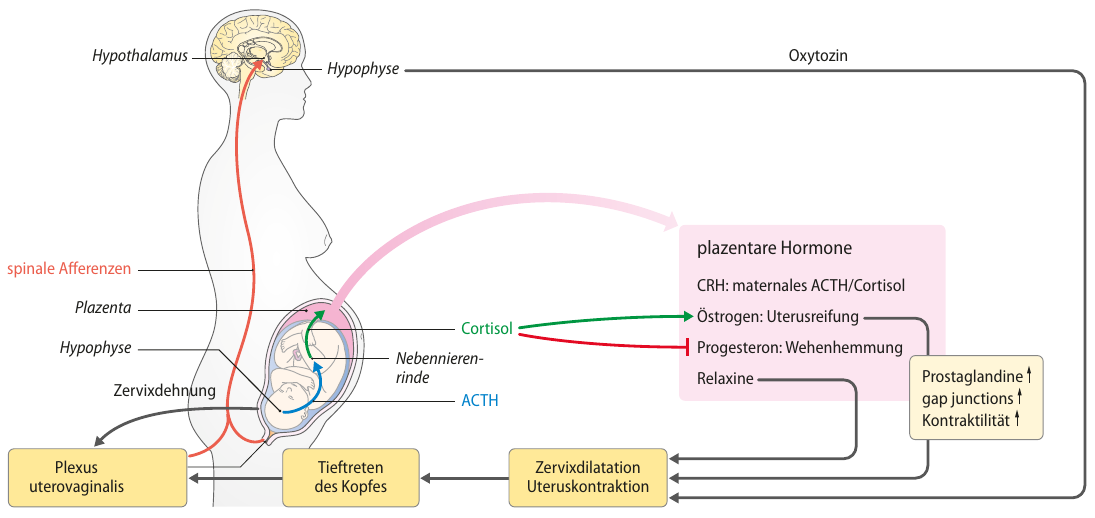
\includegraphics[width=\textwidth]{geburt_hormone}
\end{center}


\end{frame}

\begin{frame}
\frametitle{Hormonelle Regelkreise ermöglichen die Geburt. }

\begin{block}{Vorbereitung}
Hohes Östrogen am Ende der Schwangerschaft  führt zu vermehrter Bildung von Oxytozin-Rezeptoren, vermehrter Produktion von  
kontraktilen Proteinen und gap junctions. 
\end{block}

\pause
\begin{block}{Ferguson Reflex}
Ferguson Reflex: Dehnung der Zervix (durch Kopf des Kindes) bewirkt Ausschüttung von Oxytozin. Positive Rückkopplung zwischen Oxytozin und Wehen. Produktion von Relaxinen hilft, die Zervix zu dilatieren. 
\end{block}

\pause

\begin{block}{Hormonproduktion im Fötus}

Fötus produziert ACTH und Cortisol. Cortisol fördert Bildung von Östrogen und hemmt Progesteron. Produktion von  DHEA in beiden Nebennierenrinden (elterlich und im Fötus!) fördert Kontraktion des Uterus. 

 

\pause

\textcolor{theme}{Was passiert bei fötalem Stress während der Schwangerschaft? }

\end{block}

\end{frame}

\begin{frame}
\frametitle{Fötaler Stress }

Wenn der Fötus Cortisol produziert, kann es zu einer Frühgeburt kommen. 

\begin{center}
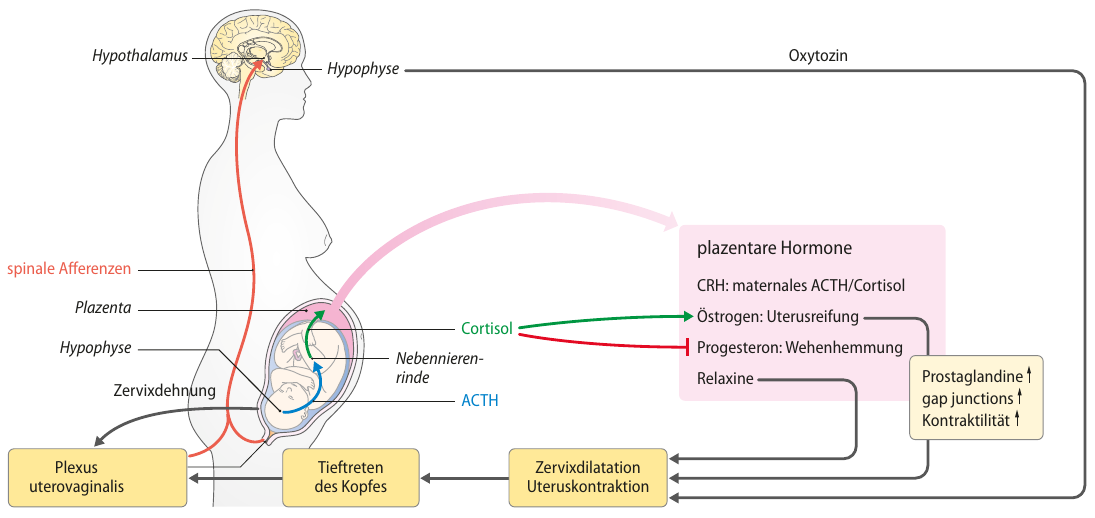
\includegraphics[width=\textwidth]{geburt_hormone}
\end{center}

\end{frame}

\section{Laktation}

%% Hormonelle Steuerung der Laktation



%% nicht Stillen ist auch ok - WHO Recommendations, Reality

%% Baby Formula Crisis



%% %% %% %% Review

\begin{frame}

 \frametitle{Jetzt* sollten Sie folgendes können}



\begin{block}{Grundlagen:}
\begin{itemize}
\item
Hormonelle Veränderungen im Verlauf der Schwangerschaft beschreiben und erklären
\item
die Entwicklung des Embryos und Fötus erklären 
\item
Körperfunktionen und Stoffaustausch des Fötus beschreiben
\item
die "Fetoplazentare Einheit" und Funktion der Plazenta erläutern
\item
den Geburtsvorgang beschreiben und erklären
\item
die hormonelle Steuerung der Laktation erklären

\end{itemize}

\end{block}



\begin{block}{Klinik:}
\begin{itemize}
\item
Erklären, wie ein Schwangerschaftstest funktioniert
\item
häufige Beschwerden und Komplikationen in der Schwangerschaft erklären

\end{itemize}

\end{block}

\end{frame}





%% %% %% %% Feedbackhinweisblock

\begin{frame}
\frametitle{Danke für Ihr Feedback!}

\begin{columns}[c]

\begin{column}{6cm}
\begin{center}
 
\includegraphics[width=\textwidth]{smilie_balloons.jpg}
\end{center}

\end{column}

\begin{column}{4cm}


\begin{center}

\includegraphics[width=\textwidth]{feedback_QR.png}
\end{center}
\end{column}


\end{columns}

\end{frame}



%% %% %% Bildnachweis
\begin{frame}
\frametitle{Bildnachweis}

\begin{tiny}
 
\begin{itemize}


\item
Bauch einer schwangeren Frau. Photo by \href{https://unsplash.com/es/@anastasiiachepinska?utm_source=unsplash&utm_medium=referral&utm_content=creditCopyText}{Anastasiia Chepinska} on \href{https://unsplash.com/s/photos/pregnancy?utm_source=unsplash&utm_medium=referral&utm_content=creditCopyText}{Unsplash}


\item
Befruchtung bis Einnistung im Menschen. Von Ttrue12, CC-BY-SA 3.0, 2012, Wikimedia Commons. 

\item
Blastozyste. Die Autorenschaft wurde nicht in einer maschinell lesbaren Form angegeben. Es wird Lennert B als Autor angenommen (basierend auf den Rechteinhaber-Angaben). - Die Autorenschaft wurde nicht in einer maschinell lesbaren Form angegeben. Es wird angenommen, dass es sich um ein eigenes Werk handelt (basierend auf den Rechteinhaber-Angaben)., Gemeinfrei, https://commons.wikimedia.org/w/index.php?curid=609008

\item
Eileiter-Ruptur. Von Ectopic\_pregnancy.svg: Hic et nuncderivative work: Hic et nunc (talk) - Ectopic\_pregnancy.svg, CC BY-SA 3.0, \url{https://commons.wikimedia.org/w/index.php?curid=17236669}

\item
Hormonelle Regelkreise während der Geburt. Aus: Friederike Werny, Stefan Schlatt. Fetomaternale Interaktion, Geburt, Laktation. In: R. Brandes et al. (Hrsg.), Physiologie des Menschen, Springer-Lehrbuch \url{https://doi.org/10.1007/978-3-662-56468-4_81}


%% %% all lectures
\item
Luftballons mit frohen und traurigen Smilies. Photo by \href{https://unsplash.com/@artbyhybrid?utm_source=unsplash&utm_medium=referral&utm_content=creditCopyText}{Hybrid} on \href{https://unsplash.com/s/photos/feedback?utm_source=unsplash&utm_medium=referral&utm_content=creditCopyText}{Unsplash}

\item
Schwangerschaftstest: Prinzip. Von Martin Brändli geändert von Klaus Hoffmeier - Eigenes Werk, CC BY-SA 2.5, \url{https://commons.wikimedia.org/w/index.php?curid=560150}




\item
Supreme Court will Recht auf Schwangerschaftsabbrüche abschaffen. Screenshot von Zeit Online, vom 3. Mai 2022.
\end{itemize}
\end{tiny}
\end{frame}





\end{document}


%%%% Columns - frequently used

%% \begin{columns}[c]
%% \begin{column}{5cm}

%% \end{column}

%% \begin{column}{5cm}

%% \end{column}
%% \end{columns}


%% Umlaute
%% Ä ä Ö ö Ü ü